% Person A's sections of the research rewrite (task S3), built on their own so
% they can be read and checked before the joint 8-page paper exists.
%
% Build:   tectonic draft_personA.tex
% Numbers: python figures/make_figures.py   (writes figures/rq3_numbers.tex and
%          figures/rq3_pooling.pdf once results/rq3_pooling.json exists; until
%          then every RQ3 number prints as ??)
%
% The preamble is a copy of ifas.tex's, so the sections drop into the joint
% paper unchanged.
\documentclass[conference]{IEEEtran}

\usepackage[T1]{fontenc}
\usepackage[utf8]{inputenc}
\usepackage{microtype}
\usepackage{cite}
\usepackage{amsmath,amssymb}
\usepackage{graphicx}
\usepackage{booktabs}
\usepackage{array}
\usepackage{xcolor}
\usepackage{tikz}
\usetikzlibrary{arrows.meta,chains,positioning,decorations.pathreplacing,calc}
\usepackage[hidelinks]{hyperref}

\graphicspath{{figures/}}

\definecolor{ink}{HTML}{1B1F3B}
\definecolor{cool}{HTML}{2A6FDC}
\definecolor{warm}{HTML}{E0602A}

\tikzset{
  >=Stealth,
  box/.style={draw=ink!65, line width=0.5pt, rounded corners=2.5pt, fill=white,
    align=center, inner xsep=4.5pt, inner ysep=4pt, minimum height=10mm,
    font=\footnotesize, text=ink},
  deep/.style={box, draw=cool!85, fill=cool!9},
  classic/.style={box, draw=warm!90, fill=warm!11},
  flow/.style={->, line width=0.55pt, draw=ink!75},
  note/.style={font=\scriptsize, text=ink!80},
}

\begin{document}

\title{Person A's sections: System, RQ3, Ethics and Limitations\\(draft for the research rewrite)}
\author{\IEEEauthorblockN{IFAS team}}
\maketitle

% System, cut to about one column for the research rewrite (task S3, Person A).
% Replaces Sections III-A to III-G of the system paper. The algorithm, the
% second-detector details and the dashboard move to an appendix or are cut.

\begin{figure*}[t]
\centering
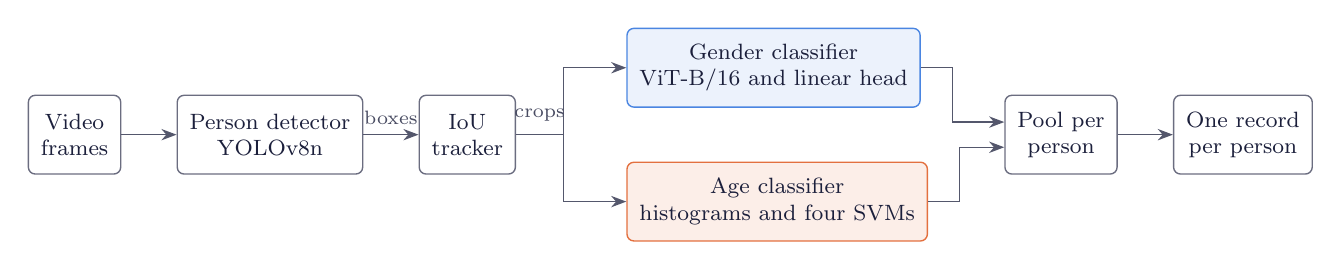
\begin{tikzpicture}[start chain=going right, node distance=7mm]
  \node[box, on chain] (video) {Video\\frames};
  \node[box, on chain] (det) {Person detector\\YOLOv8n};
  \node[box, on chain] (trk) {IoU\\tracker};
  \node[deep, right=14mm of trk, yshift=8.5mm] (gen) {Gender classifier\\ViT-B/16 and linear head};
  \node[classic, right=14mm of trk, yshift=-8.5mm] (age) {Age classifier\\histograms and four SVMs};
  \node[box, right=62mm of trk] (vote) {Pool per\\person};
  \node[box, right=7mm of vote] (rec) {One record\\per person};

  \draw[flow] (video) -- (det);
  \draw[flow] (det) -- node[note, above] {boxes} (trk);
  \draw[flow] (trk.east) -- ++(6mm,0) |- (gen.west);
  \draw[flow] (trk.east) -- ++(6mm,0) |- (age.west);
  \node[note, above=0.4mm] at ($(trk.east)+(3mm,0)$) {crops};
  \draw[flow] (gen.east) -- ++(4mm,0) |- ($(vote.west)+(0,1.6mm)$);
  \draw[flow] (age.east) -- ++(4mm,0) |- ($(vote.west)+(0,-1.6mm)$);
  \draw[flow] (vote) -- (rec);
\end{tikzpicture}
\caption{The IFAS pipeline. Each tracked person is classified on up to 12 frames
by both models, and a pooling rule turns those frames into one label per person.
RQ3 asks which pooling rule to use.}
\label{fig:pipeline}
\end{figure*}

\section{System}
\label{sec:system}
IFAS turns a video into one record per person (Fig.~\ref{fig:pipeline}).
YOLOv8n~\cite{jocher2023yolov8} finds the people in every second frame. A greedy
tracker links boxes across frames by intersection over union (IoU) and keeps a
lost track open for up to 8\,s, so a person the detector misses for a moment is
not counted twice. The tracker has no appearance model.

Two classifiers label the crops of each tracked person. Gender comes from a
ViT-B/16~\cite{dosovitskiy2021vit} with a linear head, fine-tuned on
PETA~\cite{deng2014peta}. Age comes from colour and LBP
histograms~\cite{ojala2002lbp,swain1991color} scored by one SVM per age
group~\cite{cortes1995svm}, whose margins a softmax turns into a distribution
over the four PETA groups. RQ1 and RQ3 use the released models unchanged, and
RQ2 retrains the gender model.

A person is classified at most once every 0.4\,s and at most 12 times. Frame $i$
of a person gives a probability vector $p_i$ over the classes $\mathcal{C}$ and a
vector of quality cues $q_i$ (Section~\ref{sec:rq3}). A pooling rule maps the
frames $\{(p_i, q_i)\}_{i=1}^{n}$ to one label. The product uses the majority
vote
\begin{equation}
\hat{y} = \arg\max_{c \in \mathcal{C}} \sum_{i=1}^{n}
  \mathbf{1}\!\left[\arg\max_{c'} p_i(c') = c\right],
\label{eq:majority}
\end{equation}
with a tie going to the class with the larger $\sum_i p_i(c)$.
Section~\ref{sec:rq3} compares it with four other rules and a learned baseline.

% RQ3: pooling over a track (task S3, Person A).
% Every number below comes from results/rq3_pooling.json through
% figures/rq3_numbers.tex, which make_figures.py writes. A number that does not
% exist yet prints as ?? in bold. Lines marked TODO need the results: write
% them once scripts/research/pooling_eval.py has run on the labelled clips.

\providecommand{\rqthree}[2]{%
  \ifcsname rq3/#1/#2\endcsname\csname rq3/#1/#2\endcsname\else\textbf{??}\fi}
\InputIfFileExists{figures/rq3_numbers.tex}{}{}

\section{RQ3: Which Frames Should Count?}
\label{sec:rq3}
A person in a store stays in view for many frames, and the frames differ. Some
crops are sharp and whole. Others are blurred by motion, cut off at the edge of
the frame or half hidden behind another shopper. The majority vote of
Eq.~\eqref{eq:majority} gives every crop the same say. RQ3 asks whether a rule
that trusts the good crops more names more people correctly, and whether hand
measured image quality does as well as a weighting learned from video labels.
Our hypothesis (H3) is that quality weighting beats the majority vote, with the
largest gain on people who are truncated or occluded.

\subsection{Pooling Rules}
Apart from the majority vote, every rule takes a weighted mean of the frames'
probability vectors and picks its largest entry:
\begin{equation}
\bar{p}(c) = \frac{\sum_i w_i\, p_i(c)}{\sum_i w_i}, \qquad
\hat{y} = \arg\max_{c} \bar{p}(c).
\label{eq:weighted}
\end{equation}
The rules differ only in the weights $w_i$.
\begin{itemize}
  \item \emph{Single frame.} One frame chosen at random. This is what a system
        without pooling would report.
  \item \emph{Majority vote.} Eq.~\eqref{eq:majority}, the product's rule.
  \item \emph{Mean probability.} $w_i = 1$.
  \item \emph{Confidence weighted.} $w_i = \max_c p_i(c)$, the classifier's own
        confidence in the frame.
  \item \emph{Quality weighted.} $w_i = \Pr(\mathrm{correct}_i \mid q_i)$, the
        chance that frame $i$ is classified correctly given its cues, from the
        quality model below.
\end{itemize}

\subsection{Quality Cues and the Quality Model}
The cue vector $q_i$ has seven entries, all measured when the crop is exported.
\begin{itemize}
  \item \emph{Sharpness.} The share of the crop's spectral energy at or above
        0.25 cycles per pixel, computed on a $128\times128$ grey version. Blur
        and low resolution both remove this band. The variance of the
        Laplacian~\cite{pech2000laplacian} is kept as a second sharpness cue.
  \item \emph{Motion.} Dense Farneb\"ack optical flow~\cite{farneback2003flow}
        between the crop's frame and the previous one: the mean flow magnitude
        inside the box minus the median magnitude outside every box, in pixels
        per frame. Subtracting the background removes camera shake, so what
        remains is the person's own movement, which is what blurs the crop.
  \item \emph{Truncation.} 1 if the box touches the frame border.
  \item \emph{Occlusion.} The box's largest IoU with another person's box in the
        same frame.
  \item \emph{Size and detector confidence.} The box's share of the frame area
        and the detector's score.
\end{itemize}
The quality model is a logistic regression with an L2 penalty from these cues
to whether the classifier got the crop right. The Laplacian variance and the
size enter as logarithms and the motion as $\log(1+m)$, because each spans
several orders of magnitude. Features are standardised, a cue that could not be
measured takes the training mean, and the model is fitted by Newton's method.
It is small and readable, and its coefficients show which cue matters
(Section~\ref{sec:rq3-results}).

\subsection{Learned Attention Baseline}
Video attribute recognition usually learns how to weigh frames from video
labels~\cite{chen2019temporal}. A reviewer will rightly ask how measured quality
compares with that, so we train the same kind of head on top of the frozen
per-frame features of our two classifiers: the 768-dimensional ViT feature that
the gender head reads, and the histograms that the age SVMs score. With $f_i$
the standardised feature of frame $i$,
\begin{gather}
z_i = W f_i + b, \qquad
\alpha_i = \frac{\exp\left(v^{\top}\tanh z_i\right)}
                {\sum_j \exp\left(v^{\top}\tanh z_j\right)}, \\
\hat{y} = \arg\max_c \Big[\, U \sum\nolimits_i \alpha_i z_i + u \,\Big]_c,
\end{gather}
with $z_i \in \mathbb{R}^{32}$. The head is trained with class-balanced
cross-entropy and Adam for 300 epochs with a weight decay of $10^{-3}$. It
needs a label for every training person. Quality weighting needs only crops
labelled right or wrong, and that difference in what each method asks for is
part of the comparison. MARS~\cite{zheng2016mars} with its tracklet
attributes~\cite{chen2019temporal} is the natural place to train the head. When
MARS is not available we train it with the same cross-validation folds as the
quality model.

\subsection{Protocol}
Two annotators labelled every person in the retail test clips from the crops
alone, without seeing the model's answers, and resolved their disagreements
together. Agreement before resolution is reported as Cohen's
$\kappa$~\cite{cohen1960kappa}. People either annotator marked unsure are left
out, and their number is reported.

The per-crop probabilities are the product's own, stored when the crops were
exported, so every rule pools exactly what the deployed system saw. The quality
model and the attention head are fitted with 5-fold cross-validation grouped by
person: no person's crops ever help weigh that person's own frames. The unit of
evaluation is the person. We report per-person accuracy with a 95\% bootstrap
interval over people~\cite{efron1993bootstrap} (2,000 resamples), and McNemar's
test~\cite{mcnemar1947} of each rule against the majority vote on the same
people, exact when fewer than 25 people disagree. To see how much pooling is
worth, we also draw $k = 1, \dots, 12$ of a person's crops at random (20 draws
per person) and pool only those. Last, we split people into those who are
truncated, or occluded, in at least half their crops, and the rest.

\begin{table}[t]
\caption{Per-person accuracy of each pooling rule with its 95\% interval over
people, and McNemar's $p$ against the majority vote. Gender: \rqthree{gender}{n}
people, age: \rqthree{age}{n} people.}
\label{tab:rq3}
\centering
\begin{tabular}{@{}lcccc@{}}
\toprule
Rule & Gender & $p$ & Age & $p$ \\
\midrule
Single frame        & \rqthree{gender}{single}     & \rqthree{gender}{p-single}     & \rqthree{age}{single}     & \rqthree{age}{p-single} \\
Majority vote       & \rqthree{gender}{majority}   & --                             & \rqthree{age}{majority}   & -- \\
Mean probability    & \rqthree{gender}{mean}       & \rqthree{gender}{p-mean}       & \rqthree{age}{mean}       & \rqthree{age}{p-mean} \\
Confidence weighted & \rqthree{gender}{confidence} & \rqthree{gender}{p-confidence} & \rqthree{age}{confidence} & \rqthree{age}{p-confidence} \\
Quality weighted    & \rqthree{gender}{quality}    & \rqthree{gender}{p-quality}    & \rqthree{age}{quality}    & \rqthree{age}{p-quality} \\
Learned attention   & \rqthree{gender}{attention}  & \rqthree{gender}{p-attention}  & \rqthree{age}{attention}  & \rqthree{age}{p-attention} \\
\bottomrule
\end{tabular}
\end{table}

\begin{figure*}[t]
\centering
\IfFileExists{figures/rq3_pooling.pdf}{%
  \includegraphics[width=\textwidth]{figures/rq3_pooling.pdf}}{%
  \fbox{\parbox{0.9\textwidth}{\centering\vspace{6mm}This figure is drawn by
  make\_figures.py once results/rq3\_pooling.json exists.\vspace{6mm}}}}
\caption{RQ3 on the retail test clips. (a) Per-person accuracy of each pooling
rule with its 95\% interval over people. (b) Accuracy when only $k$ of a
person's crops are pooled.}
\label{fig:rq3}
\end{figure*}

\subsection{Results}
\label{sec:rq3-results}
Table~\ref{tab:rq3} and Fig.~\ref{fig:rq3} give the results. With no pooling,
a single frame gave a per-person gender accuracy of
\rqthree{gender}{single-value}. The majority vote reached \rqthree{gender}{majority-value} and quality weighting
\rqthree{gender}{quality-value} (McNemar $p = \rqthree{gender}{p-quality}$, with
\rqthree{gender}{b-quality} people right only under quality weighting and
\rqthree{gender}{c-quality} right only under the vote). For age the same three
numbers were \rqthree{age}{single-value}, \rqthree{age}{majority-value} and
\rqthree{age}{quality-value}.
% TODO after results: one sentence on whether H3 holds for gender and for age.

On the \rqthree{gender}{truncated-n} people who were truncated in most of their
crops, the vote reached \rqthree{gender}{truncated-majority} and quality
weighting \rqthree{gender}{truncated-quality}. On the \rqthree{gender}{occluded-n}
occluded people the two reached \rqthree{gender}{occluded-majority} and
\rqthree{gender}{occluded-quality}.
% TODO after results: is the gain larger on these subsets, as H3 predicts?

The learned attention head reached \rqthree{gender}{attention-value} on gender
and \rqthree{age}{attention-value} on age, trained with
\rqthree{gender}{attention-fitted}. Its frame weights and the quality weights had a mean
Spearman correlation of \rqthree{gender}{rho} for gender.
% TODO after results: if rho is high, the head learned roughly what the cues
% measure; if low, it attends to something else. Say which, and what follows
% for a deployment that has no video labels.

In the gender quality model fitted on all people, the standardised coefficients
were \rqthree{gender}{coef-hf_ratio} for sharpness,
\rqthree{gender}{coef-log1p_motion} for motion, \rqthree{gender}{coef-truncated}
for truncation and \rqthree{gender}{coef-occlusion} for occlusion. A positive
coefficient means crops with more of that cue are classified correctly more
often.
% TODO after results: name the cue that matters most, and say if any sign is
% the opposite of what one would expect.

Fig.~\ref{fig:rq3}b shows how accuracy grows with the number of frames pooled.
% TODO after results: where the curve flattens. If it flattens well before 12,
% the vote cap could be lowered and the classifier run less often.

% Ethics (task S3, Person A). Keep this section in the 8-page version: a paper
% that films shoppers and guesses their gender and age has to say this.
% Every sentence here is a claim about how the clips were collected. Before
% submitting, check each one against docs/research-data.md and the signed
% letters, and change or cut any that did not hold.

\section{Ethics}
\label{sec:ethics}
The retail clips are CCTV recordings of members of the public, and the study
estimates attributes of those people. We set the following rules before
recording anything, and kept to them.

\emph{Permission.} Every clip comes from a store that gave written permission
for this study. The letter says what footage is used, what is done with it, how
long it is kept and that the store can withdraw at any time. The footage comes
from the store's existing cameras, which are signposted. We installed no camera
and recorded nothing new.

\emph{Privacy.} Footage, crops and labels stay on the project's own machines and
are never published or shared. No figure in this paper shows a recognisable
person. We do not identify anyone, and the system stores no face template or
any other means to find a person again in other footage. Results are reported
as totals over people.

\emph{Labels.} The annotators recorded apparent gender and an apparent age group
from the crops. These are judgements about appearance and say nothing about how
a person identifies. Gender is recorded as two classes because PETA and MARS
label it that way. This is a limitation of the data, and a deployment should
report it as an estimate of appearance. Children are not labelled: the age
model's youngest group starts at 16, PETA's under-15 group is left out of its
training, and no person who looked under 16 in the retail clips was labelled.

\emph{Use.} The system counts and describes groups of shoppers so a store can
plan staffing and layout. It is not meant to treat individual customers
differently, and should not be used that way. Gender and age estimates are
wrong for a measurable share of people, which Section~\ref{sec:rq3} reports.
They are not fit for any decision about an individual.

% Limitations (task S3, Person A). Items about RQ1 and RQ2 belong to Person B
% and go in the marked place before this goes into the paper.

\section{Limitations}
\label{sec:limits}
\begin{itemize}
  \item \emph{Few stores.} The retail clips come from a small number of cameras
        in a small number of stores. The intervals in Section~\ref{sec:rq3} cover
        the variation between people, not between stores, and a store with
        different lighting or camera placement may behave differently.
  \item \emph{Labels are judgements.} The ground truth is what two annotators
        saw in the crops. People they marked unsure are left out, which removes
        the hardest cases from every accuracy we report.
  \item \emph{Correlated frames.} Crops of one person taken 0.4\,s apart share
        lighting, pose and clothing, so their errors are not independent. Pooling
        cannot fix an error that every frame makes, and accuracy against the
        number of frames pooled shows how much independent evidence the frames
        really hold.
  \item \emph{Hand-chosen cues.} The quality model sees seven cues that we chose.
        A failure that none of them measures, such as a bag held in front of the
        body or strong backlight, gets no lower weight.
  % If the MARS images are obtained and used (--attention-train), rewrite this item.
  \item \emph{Small training sets.} With MARS unavailable, the quality model and
        the attention head were fitted on the retail people themselves, with
        cross-validation. Both would likely improve with more data, and the
        attention head, with far more parameters, more so.
  \item \emph{The tracker.} Pooling is only as good as the track it pools. The
        tracker has no appearance model, so two people who cross paths can swap
        tracks, and a pooled label can then mix two people.
  % Person B: add the RQ1 and RQ2 limitations here (PETA split, single store as
  % FDA target, seeds).
\end{itemize}


\bibliographystyle{IEEEtran}
\bibliography{refs}

\end{document}
